\documentclass{beamer}
\usetheme{Madrid}

\usepackage{tikz}
\usepackage{amsmath}
\usepackage{amsthm}
\tikzstyle{vertex}=[
	draw=black,
	shape=circle,
	fill=blue,
	minimum size=15pt,
	inner sep=0pt
]
\tikzstyle{edge} = [draw,very thick,-]
\tikzstyle{pstyle} = [very thick]
\tikzstyle{highlight} = [ultra thick]
\tikzstyle{iso} = [very thick,color=red]

\title{Spanning Star Forest Problem}
\author{Adam Starak}
\begin{document}
\begin{frame}[plain]
    \maketitle
\end{frame}

\begin{frame}{Star definition}

\begin{block}{Definition}
	A star is a tree of size at least 2 for which at most one vertex has a degree greater than 1.
\end{block}

\begin{Examples}<2->
	\begin{columns}
		\begin{column}{0.33\textwidth}<2->
			\centering
			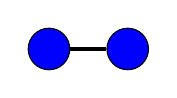
\begin{tikzpicture}[node distance=1cm]
				
				\node[vertex]	(A)	{};
				\node[vertex]	(B) [right of=A]{};
				
				\path[pstyle] (A) edge node {} (B);
				
			\end{tikzpicture}
		\end{column}
		\begin{column}{0.33\textwidth}<3->
			\centering
			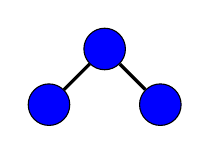
\begin{tikzpicture}[node distance=1cm]
			
			\node[vertex]	(A)	{};
			\node[vertex]	(B) [below right of=A]{};
			\node[vertex]	(C) [below left of=A]{};
			
			\path[pstyle]
				(A) edge node {} (B)
				(A) edge node {} (C);
			
			\end{tikzpicture}
		\end{column}
		\begin{column}{0.33\textwidth}<4->
			\centering
			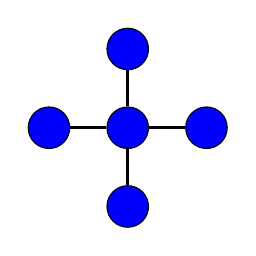
\begin{tikzpicture}[node distance=1cm]
			
			\node[vertex]	(A)	{};
			\node[vertex]	(B) [right of=A]{};
			\node[vertex]	(C) [left of=A]{};
			\node[vertex]	(D) [below of=A]{};
			\node[vertex]	(E) [above of=A]{};
			
			\path[pstyle] 
				(A) edge node {} (B)
				(A) edge node {} (C)
				(A) edge node {} (D)
				(A) edge node {} (E);
			
			\end{tikzpicture}
		\end{column}
	\end{columns}

\end{Examples}

\end{frame}



\begin{frame}{Spanning Star Forest Problem}
	\begin{block}{Definition}
		Given a graph $G$ decide whether it has a \emph{Spanning Star Forest}.
	\end{block}
\end{frame}

\begin{frame}{Example}
	\centering
	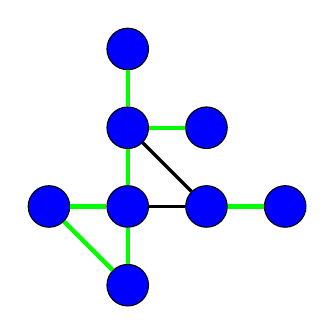
\begin{tikzpicture}[node distance=1cm]
		
		\node[vertex]	(A)	{};
		\node[vertex]	(B) [below of=A]{};
		\node[vertex]	(C) [right of=B]{};
		\node[vertex]	(D) [below of=B]{};
		\node[vertex]	(E) [left of=D]{};
		\node[vertex]	(F) [right of=D]{};
		\node[vertex]	(G) [right of=F]{};
		\node[vertex]	(H) [below of=D]{};
		
		\path[pstyle]<1->
		(A) edge node {} (B)
		(B) edge node {} (C)
		(B) edge node {} (D)
		(B) edge node {} (F)
		(D) edge node {} (E)
		(D) edge node {} (H)
		(D) edge node {} (F)
		(F) edge node {} (G)
		(E) edge node {} (H);
		
		\path[highlight, green]<2>
			(A) edge node {} (B)
			(B) edge node {} (C)
			(B) edge node {} (D)
			(E) edge node {} (H)
			(F) edge node {} (G);
			
		\path[highlight, green]<3>
			(A) edge node {} (B)
			(B) edge node {} (C)
			(D) edge node {} (E)
			(D) edge node {} (H)
			(F) edge node {} (G);
	
	\end{tikzpicture}
\end{frame}

\begin{frame}{Spanning Star Forest Problem}
	\begin{block}{Lemma }
		$G$ contains a Spanning Star Forest if and only if it does not contain any isolated vertices.
	\end{block}

	\bigskip

	\onslide<2>{
		\textbf{Forward implication}. Trivial, Every vertex belongs to a tree of size at least 2. Thus, it's degree is at least 1.
	}
\end{frame}

\begin{frame}[t]{Backward implication}
	\begin{columns}
		
		\begin{column}{0.75\textwidth}
			\small
			\begin{itemize}[<+->]
				\setlength{\leftmargini}{2pt}
				\item[] Suppose $G$ has no isolated vertices.
				\item[] Induction by the number of vertices in $G$.
				\bigskip
				\item[] Let $n=2$.
				\item[] Graph is a correct Spanning Star Forest.
			\end{itemize}
		\end{column}
		\begin{column}{0.25\textwidth}
			\onslide<4>{
				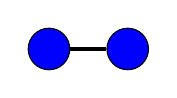
\begin{tikzpicture}[node distance=1cm]
					
					\node[vertex]	(A)	{};
					\node[vertex]	(B) [right of=A]{};
					
					\path[pstyle]<1->
					(A) edge node {} (B);
				
				\end{tikzpicture}
			}
		\end{column}
	\end{columns}
\end{frame}

\begin{frame}[t]{Backward implication}
	\begin{columns}
		\begin{column}{0.6\textwidth}
			\small
			\begin{itemize}
				\setlength{\leftmargini}{2pt}
				\item[]<1-> Suppose $G$ has no isolated vertices.
				\item[]<1-> Induction by the number of vertices in $G$.
				\bigskip
				\item[]<1-> Inductive step.
				\item[]<2-> Assume the condition holds for all graphs of size at most $n$.
				\item[]<3-> Suppose there does not exist a vertex $v$ such that $G \setminus \{v\}$ has no isolated vertices.
				\item[]<4-> Graph $G$ is a correct Spanning Star Forest.
			\end{itemize}
		\end{column}
		\begin{column}{0.4\textwidth}
			\centering
			\onslide<4>{
				\def\lastx{F}
				\begin{tikzpicture}[node distance=1cm]
				
				\foreach \x [remember=\x as \lastx] in {A,...,D} 
				{
					\node[vertex] (\x) 	[below of=\lastx]{};
					\node[vertex] (\x\x)	[right of=\x]{}; 
					\path[pstyle] (\x) edge node {} (\x\x);
				}
				
				
				\end{tikzpicture}
			}
		\end{column}
	\end{columns}
\end{frame}

\begin{frame}[t]{Backward implication}
\begin{columns}
	\begin{column}{0.6\textwidth}
		\small
		\begin{itemize}
			\setlength{\leftmargini}{2pt}
			\item[]<1-> Suppose $G$ has no isolated vertices.
			\item[]<1-> Induction by the number of vertices in $G$.
			\bigskip
			\item[]<1-> Inductive step.
			\item[]<1-> Assume the condition holds for all graphs of size at most $n$.
			\item[]<1-> Suppose there exists a vertex $v$ such that $G \setminus \{v\}$ has no isolated vertices.
			\item[]<2-> Let $S$ be a solution for a graph $G \setminus \{v\}$.
			\item[]<3-> Now, let's try to add vertex $v$ to the solution $S$.
		\end{itemize}
	\end{column}
	\begin{column}{0.4\textwidth}
		\onslide<4->{
			\def\lastx{A}
			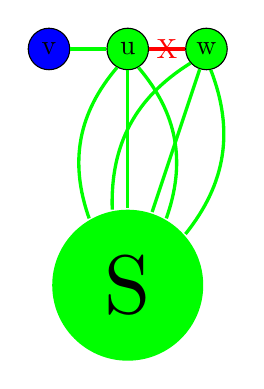
\begin{tikzpicture}[node distance=1cm]
			
			\tikzstyle{state}=[fill=blue,shape=circle,scale=1.5]
			\tikzstyle{solution}=[fill=green,shape=circle,scale=3]
			
			\node[vertex] 	(A) 				{v};
			\node[vertex,fill=green] 	(B) [right of=A]	{u};
			\node[vertex,fill=green] 	(C) [right of=B]	{w};
			\node[solution]	(D)	[below of=B]	{S};
			
			\path[pstyle]<4>
				(A) edge node {} (B);
			
			\path[pstyle, green]<-8>
				(B) edge node {} (C);
				
			\path[highlight, green]<5>
				(A) edge node {} (B);
			
			
			
			\path[pstyle, green]<6-7>
				(B) edge node {} (D)
				(B)[bend left] edge node {} (D)
				(B)[bend right] edge node {} (D);
			
			\path[pstyle]<6>
				(A) edge node {} (B);
				
			\path[highlight,green]<7>
				(A) edge node {} (B);
				
				
				
			\path[pstyle,green]<8-9>
				(C) edge node {} (D)
				(C)[bend left] edge node {} (D)
				(C)[bend right] edge node {} (D);
			
			\path[pstyle]<8>
				(A) edge node {} (B);
			
			\path[highlight,green]<9>
				(A) edge node {} (B);
				
			\path[pstyle,red]<9>
				(B) edge node {X} (C);
					
			\end{tikzpicture}
		}
	\end{column}
\end{columns}
\end{frame}

\begin{frame}{Parametrization by the number of stars}

\begin{block}{Definition}
	Given a pair $(G,k)$ find a Spanning Star Forest $S$ such that $S$ has at most $k$ connected components.
\end{block}

\bigskip

\begin{block}{Dominating Set}<2->
	Given a pair $(G,k)$ find a set $D \subseteq V(G)$ such that $|D| \leq k$ and every node is either in $D$ or adjacent to $D$.
\end{block}

\bigskip

\onslide<3>{The problem is NP-Complete}

\end{frame}

\begin{frame}{NP-completeness - membership in NP}
	Trivial. Given $S$ check if it is a Spanning Star Forest and if it has at most $k$ connected components.
\end{frame}

\begin{frame}{NP-completeness - hardness}
\textbf{Construction}:
\onslide<2->{Let $(G,k)$ be an instance of Dominating Set Problem.\\}
\bigskip
\onslide<3->{We create $G'$ as follows: for every isolated vertex $v$ introduce a vertex $v'$ and an edge $(v,v')$.}

\begin{Lemma}<4->
	$(G,k)$ has a solution if and only if $(G',k)$ has one.
\end{Lemma}

\onslide<5->{
	\textbf{Backward implication}. \\
	Set of centers represents a correct dominating set of $G$.
}

\end{frame}

\begin{frame}[t]{NP-completeness: Forward implication}
	\begin{columns}
		\begin{column}{0.6\textwidth}
			\small
			\setlength{\leftmargini}{2pt}
			\begin{itemize}[<+->]
				\item[] \textbf{Forward implication}.
				\item[] Without a loss of generality, if there exists a solution for $(G,k)$, then there exists a solution of minimal size. Let $D$ be such a solution.
				\item[] We create solution $S$ as follows: For every $v \in V(G') \setminus D$ add an edge $(v,u)$ to the solution where $u \in D$.
				\item[] Assume $S$ contains an isolated vertex. Trivially, $v \in D$.
				
			\end{itemize}
		\end{column}
		\begin{column}{0.4\textwidth}
			\def\lastx{A}
			\centering
			\begin{tikzpicture}[node distance=1cm]
			
				\tikzstyle{dominating} = [fill=red]
				\tikzstyle{dominated} = [fill=green]
				
				\only<5>
				{
					\node[vertex,dominating]	(A)	 				{v};
					\node[vertex,dominating]	(B) [right of=A]	{u};
					
					\path[pstyle]
						(A) edge node {} (B);
				}	
				
				\only<6>
				{
					\node[vertex,dominating]	(A)	 				{v};
					\node[vertex,dominated]		(B) [right of=A]	{u};
					\node[vertex,dominating]	(C) [right of=B]	{w};
					
					\path[pstyle]
					(A) edge node {} (B)
					(B) edge node {} (C);	
				}
				
				\only<7-8>
				{
					\node[vertex,dominating,]	(A)	 				{v};
					\node[vertex,dominated,]	(B) [right of=A]	{u};
					\node[vertex,dominating,]	(C) [right of=B]	{w};
					\node[vertex,dominated,]	(D)	[above of=C]	{z};
					
					\path[pstyle]
					(A) edge node {} (B)
					(B) edge node {} (C)
					(C) edge node {} (D);
					
					\path[pstyle,red]<8>
					(B) edge node {X} (C);
					
				}
			
			\end{tikzpicture}
		\end{column}
	\end{columns}
\end{frame}

\begin{frame}{Reduction from SSF to Dom-Set}
	\begin{block}{Construction}
		Given $(G,k)$ transform the instance as following:
		
		\begin{equation*}
			(G',k') =
			\begin{cases}
				(G,0), & \text{if } G \text{ contains an isolated vertex}. \\
				(G,k), & \text{otherwise.}
			\end{cases}
		\end{equation*}
		
	\end{block}
\end{frame}

\begin{frame}{Spanning Star Forest Extension Problem}
	\begin{block}{Definition}
		Given a graph $G$ and a set of edges $F \subseteq E(G)$, find a Spanning Star Forest $S$ such that $F \subseteq E(S)$.
	\end{block}

	\begin{Example}
		\begin{center}
			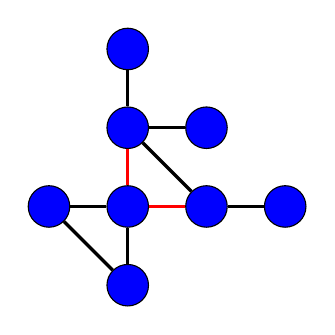
\begin{tikzpicture}[node distance=1cm]
			
				\tikzstyle{state}=[fill=blue,shape=circle]
				
				\node[vertex]	(A)	{};
				\node[vertex]	(B) [below of=A]{};
				\node[vertex]	(C) [right of=B]{};
				\node[vertex]	(D) [below of=B]{};
				\node[vertex]	(E) [left of=D]{};
				\node[vertex]	(F) [right of=D]{};
				\node[vertex]	(G) [right of=F]{};
				\node[vertex]	(H) [below of=D]{};
				
				\path[pstyle]
				(A) edge node {} (B)
				(B) edge node {} (C)
				(B) edge node {} (D)
				(B) edge node {} (F)
				(D) edge node {} (E)
				(D) edge node {} (H)
				(E) edge node {} (H)
				(F) edge node {} (G);
				
				\path[pstyle, red]
				(B) edge node {} (D)
				(D) edge node {} (F);
			
			\end{tikzpicture}
		\end{center}
		
	\end{Example}
\end{frame}

\begin{frame}[t]{Instance normalization}
	\begin{columns}
		\begin{column}{0.6\textwidth}
			\small
			\begin{itemize}[<+->]
				\item[(R1)] If $G$ has an isolated vertex, it is a no instance.
				\item[(R2)] If $G$ has a path of size 3 made from isolated edges, then it is a no instance
				\item[(R3)] If $G$ has a path of size 2 made from isolated edges, then remove all the vertices adjacent to the center.
			\end{itemize}
		\end{column}
			\begin{column}{0.4\textwidth}
				\def\lastx{A}
				\only<2>{
					\centering
					\begin{tikzpicture}[node distance=1cm]
						
						\node[vertex] (A) {};
						
						\foreach \x [remember=\x as \lastx] in {B,C,D}
						{
							\node[vertex] (\x) [above of=\lastx] {};
							\path[iso] (\lastx) edge node {} (\x);
						}
					\end{tikzpicture}
				}
				\only<3>{
					\centering
					\begin{tikzpicture}[node distance=1cm]
						
						\node[vertex] (A) {};
						
						\foreach \x [remember=\x as \lastx] in {B,C}
						{
							\node[vertex] (\x) [above of=\lastx] {};
							\path[iso] (\lastx) edge node {} (\x);
						}
						
						\node[vertex] (D) [above right of=B] {};
						\node[vertex] (E) [right of=B] {};
						\node[vertex] (F) [below right of=B] {};
						
						\path[pstyle]
							(B) edge node {} (D)
							(B) edge node {} (E)
							(B) edge node {} (F);
					\end{tikzpicture}
				}
			\end{column}
	\end{columns}
\end{frame}


\begin{frame}[t]{Instance normalization 2}
	\small
	\setlength{\leftmargini}{2pt}
	\begin{itemize}
		\item[] {
			\begin{color}{red}
				$G_{P}$
			\end{color}
			$= \{v: u,v \notin V(F)$ and $\exists (u,v) \in E(G)\}$.
		}
		\item[] {
			\begin{color}{green}
				$G_{NP}$
			\end{color}
			$ = G \setminus G_P.$
		}
	\end{itemize}

	\onslide<3> {
		$G_P$ has always a SSF because it does not contain any isolated edges and for all $v \in V(G_P)$ $deg_{G_P}(v) \neq 0$.
	}

	\vfill    
	\def\lastx{A}
	\centering
	\begin{tikzpicture}[node distance=2cm]
		
		\node[vertex] (A){};
		
		\foreach \x [remember=\x as \lastx] in {B,...,F} {
			\node[vertex]	(\x)	[right of=\lastx]		{};
		};

		\foreach \x in {A,B,D,E} {
			\node[vertex] (\x\x)	[above right of=\x]	{};
		}
	
		\node[vertex] (AAA) [above right of=AA] {};
		
		\path[iso]
			(A) edge node {} (B)
			(C) edge node {} (D)
			(E) edge node {} (F);
		
		\path[pstyle]
			(AA) edge node {} (AAA)
			(BB) edge node {} (AAA)
			(BB) edge node {} (DD)
			(EE) edge node {} (E)
			(DD) edge node {} (E)
			(DD) edge node {} (D)
			(AA) edge node {} (A)
			(AA) edge node {} (B)
			(AA) edge node {} (C)
			(BB) edge node {} (E)
			(BB) edge node {} (D)
			(BB) edge node {} (C);
			
		\only<2->{
			\node[vertex,fill=green] (A){};
			\def\lastx{A}
			\foreach \x [remember=\x as \lastx] in {B,...,F} {
				\node[vertex,fill=green] (\x) [right of=\lastx] {};
			};
			
			\foreach \x in {A,B,D} {
				\node[vertex,fill=red] (\x\x)	[above right of=\x]	{};
			}
			
			\node[vertex,fill=red] (AAA) [above right of=AA] {};
			\node[vertex,fill=green] (EE) [above right of=E] {};
		}
			
	
	\end{tikzpicture}
	
\end{frame}

\begin{frame}[t]{Instance normalization 3}
	\small
	\setlength{\leftmargini}{2pt}
	\begin{itemize}
		\item[] {
			\begin{color}{red}
				$G_{P}$
			\end{color}
			$= \{v: u,v \notin V(F)$ and $\exists (u,v) \in E(G)\}$.
		}
		\item[] {
			\begin{color}{green}
				$G_{NP}$
			\end{color}
			$ = G \setminus G_P.$
		}
	\end{itemize}
	\begin{Lemma}
		$(G,F)$ has a solution if and only if $(G_{NP},F)$ has one.
	\end{Lemma}
	\only<2-6>{
		\begin{itemize}[<+(1)->]
			\item[] \textbf{Backward implication}.
			\item[] Let $S$ be a solution for $G_{NP}$.
			\item[] Partition $G$ into $(G_P, G_{NP})$.
			\item[] Find a solution $S'$ for $G_P$.
			\item[] $S \cup S'$ is a solution for $G$.
		\end{itemize}
	}
	\onslide<7> {
		\textbf{Forward implication}.
		\bigskip
		
		\def\lastx{A}
		\centering
		\begin{tikzpicture}[node distance=2cm]
		
			\node[vertex,fill=green] (A){};
			\def\lastx{A}
			\foreach \x [remember=\x as \lastx] in {B,...,F} {
				\node[vertex,fill=green] (\x) [right of=\lastx] {};
			};
			
			\foreach \x in {A,B,D} {
				\node[vertex,fill=red] (\x\x)	[above right of=\x]	{};
			}
			
			\node[vertex,fill=red] (AAA) [above right of=AA] {};
			\node[vertex,fill=green] (EE) [above right of=E] {};
			
			\path[pstyle]
			(AA) edge node {} (AAA)
			(BB) edge node {} (AAA)
			(BB) edge node {} (DD)
			(EE) edge node {} (E)
			(DD) edge node {} (E)
			(DD) edge node {} (D)
			(AA) edge node {} (A)
			(AA) edge node {} (B)
			(AA) edge node {} (C)
			(BB) edge node {} (E)
			(BB) edge node {} (D)
			(BB) edge node {} (C);
			
			\path[iso]
			(A) edge node {} (B)
			(C) edge node {} (D)
			(E) edge node {} (F);
			
		\end{tikzpicture}}
\end{frame}

\begin{frame}[t]{SSFE is NP-complete}
	\begin{block}{Membership in NP}<2->
		Trivial. Given a solution $S$ check if all isolated edges are included and if it is a correct SSF.
	\end{block}
\end{frame}

\begin{frame}[t]{SSFE - Hardness}
	\onslide<2->{
		\textbf{Reduction from 3-SAT}: Given formula $\phi$ do the following.
	}
	\begin{enumerate}[<+(3)->]
		\item For each variable $x_i$ introduce vertices $v_{x_i}$, $v_{\neg x_i}$.
		\item For each $v_{x_i}$, $v_{\neg x_i}$ introduce an isolated edge.
		\item For each clause $c_i$ introduce vertex $v_{c_i}$.
		\item If literal $l$ exists in clause $c$ introduce an edge between them.
	\end{enumerate}

	\onslide<3->{
		\begin{center}
			$(x_1 \lor x_2 \lor \neg x_4) \land (\neg x_1 \lor x_3 \lor \neg x_5) \land (x_4 \lor x_5 \lor \neg x_1)$
		\end{center}
	}

	\centering
	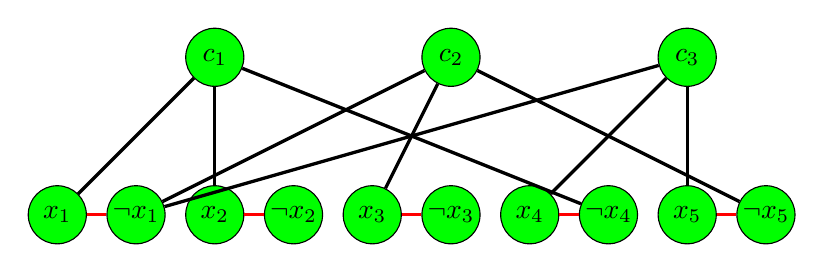
\begin{tikzpicture}[node distance=1cm]
		\tikzstyle{big} = [fill=green, minimum size=21pt]
		
		\onslide*<4->{
			
			\node[vertex,big] (A)				  {$x_1$};
			\node[vertex,big] (AA)	[right of=A]  {$\neg x_1$};
			\node[vertex,big] (B)	[right of= AA] {$x_2$};
			\node[vertex,big] (BB)	[right of=B]  {$\neg x_2$};
			\node[vertex,big] (C)	[right of=BB] {$x_3$};
			\node[vertex,big] (CC)	[right of=C]  {$\neg x_3$};
			\node[vertex,big] (D)	[right of=CC] {$x_4$};
			\node[vertex,big] (DD)	[right of=D]  {$\neg x_4$};
			\node[vertex,big] (E)	[right of=DD] {$x_5$};
			\node[vertex,big] (EE)	[right of=E]  {$\neg x_5$};
		}
		
		\onslide<5-> {
			\foreach \x in {A,B,C,D,E} {
				\path[pstyle,red] (\x) edge node {} (\x\x);
			}
		}
		
		\onslide<6-> {
			\node (XX) [above of=B] {};
			\node (YY) [above of=CC] {};
			\node (ZZ) [above of=E] {};
			\node[vertex,big] (X) [above of=XX] {$c_1$};
			\node[vertex,big] (Y) [above of=YY] {$c_2$};
			\node[vertex,big] (Z) [above of=ZZ] {$c_3$};
		}
	
		\onslide<7-> {
			\path[pstyle]
				(A) edge node {} (X)
				(B) edge node {} (X)
				(DD) edge node {} (X)
				(AA) edge node {} (Y)
				(C) edge node {} (Y)
				(EE) edge node {} (Y)
				(D) edge node {} (Z)
				(E) edge node {} (Z)
				(AA) edge node {} (Z);
		}
		
	\end{tikzpicture}
	
\end{frame}

\begin{frame}{SSFE reverse reduction}
	\begin{block}<2->{Theorem}
		There exists a reduction from 3-SAT to SSFE.
	\end{block}

	\bigskip

	\begin{block}<3->{Corollary}
		3-SAT and SSFE are equally hard
	\end{block}
\end{frame}

\begin{frame}[t]{Parametrizations}
\begin{itemize}[<+(1)->]
	\item[] Number of isolated edges $|F|$.
	\bigskip
	\item[] Number of vertices $|V(G) \setminus V(F)|$.
	\bigskip
	\item[] Treewidth.
\end{itemize}
\end{frame}

\begin{frame}[t]{Number of isolated edges $|F|$}
	\begin{block}<2->{Simple algorithm}
		\setlength{\leftmargini}{2pt}
		\begin{itemize}[<+(1)->]
			\item[] Branch on every isolated edge and check whether chosen vertices form a Spanning Star forest.
			\item[] Complexity: $\mathcal{O}^*(2^{|F|})$.
		\end{itemize}
	\end{block}
	\bigskip
	\begin{block}{SETH}<4->
		let $\delta_q$ be the infinimum of the set of constants $c$ for which there exists an algorithm solving q-SAT in time $\mathcal{O}^*(2^{cn})$. Then:\bigskip
		\begin{center}
			$\lim\limits_{q \rightarrow \infty } \delta_q = 1$
		\end{center}
	\end{block}
	\onslide
\end{frame}

\begin{frame}[t]{SSFE parameterized by $|F|$ doesn't invoke kernel.}
	\small
	\begin{block}<2->{Proving nonexistence of a kernel}
		\setlength{\leftmargini}{2pt}
		\begin{itemize}[<+(1)->]
			\item[] Input: $(x_1,k),(x_2,k),...,(x_t,k)$ where $(x_i,k)$ - instance of a given problem $Q$.
			\item[] Question: Does there exist an instance $(x',k)$ such that satisfies the following conditions:
			\item[] (1) $k' \leq poly(\max |(x_i,k)| + log(t))$
			\item[] (2) $(x',k') \in Q$ if and only if $(x_i,k) \in Q$ for some $i \leq t$.
		\end{itemize}
	\end{block}
	\onslide<6->{
		For a more general idea, read chapter 15 from Parameterized Algorithms.
		\bigskip
		\begin{Example}<7->
			Given instances $(G_1,k),(G_2,k),...,(G_t,k)$ of k-Path problem return $(\bigcup_{i=1}^t G_i,k)$
		\end{Example}
	}
\end{frame}

\begin{frame}{SSFE parameterized by $|F|$ doesn't invoke kernel - Proof}
	\huge\centering
	Proof on the board.
\end{frame}

\begin{frame}[t]{SSFE parameterized by $|V(G)| \setminus |V(F)|$}
	\begin{block}<2->{Quadratic kernel}
		If there exists a vertex $v \in V(G) \setminus V(F)$ such that $deg_G(v) > k$, then remove $v$.
	\end{block}
	\setlength{\leftmargini}{2pt}
	\begin{itemize}[<+(2)->]
		\item[] \textbf{Proof}:
		\item[] Assume there exists a SSF $S$ in $G \setminus \{v\}$.
		\item[] Then, we "set" at most $k$ centers.
		\item[] In graph $G$ $deg_G(v)>k$. So, there exists isolated edge $(u,w)$ such that $deg_S(u)=deg_S(w)=1$ and either $(v,u) \in E(G)$ or $(v,w) \in E(G)$.
		\bigskip
		\item[] Number of edges: $\leq 2k^2$
		\item[] Number of edges: $\leq k + 2k^2$.
	\end{itemize}
\end{frame}

\end{document}
